% !TeX root = ../main.tex
% A–L 22:8, 23:1–3; M–Z 22:6–9.
\section{Simmetrie di un poligono regolare}
Per $n\ge3$, il \textbf{gruppo diedrale} $D_n$ è il gruppo delle isometrie del piano che mandano un poligono regolare di $n$ lati in sé, con la composizione. Numerando i vertici in senso antiorario, ogni simmetria induce una permutazione. Questa assegnazione rispetta la composizione ed è iniettiva: le immagini di tre vertici non allineati determinano un'isometria, perché un punto è determinato dalle distanze da tre punti non allineati.

\begin{proposizione}
Siano $r$ la rotazione antioraria di $2\pi/n$ e $s$ una riflessione del poligono.
\begin{enumerate}
\item $r$ ha ordine $n$, $s$ ha ordine $2$ e $srs^{-1}=r^{-1}$.
\item Ogni elemento si scrive in modo unico $r^i s^j$, con $0\le i<n$ e $j\in\{0,1\}$. Quindi $D_n=\langle r,s\rangle$ ha ordine $2n$.
\end{enumerate}
\end{proposizione}
\begin{proof}
\textbf{1.} Sui vertici numerati ciclicamente, $r$ avanza di una posizione. La riflessione inverte il verso di percorrenza e applicata due volte fissa ogni vertice. Riflettere, avanzare e riflettere di nuovo arretra di una posizione.

\textbf{2.} Una simmetria sceglie l'immagine del primo vertice ($n$ possibilità) e il verso in cui percorrere i lati (due possibilità). Questi dati determinano le immagini di tutti i vertici. Le $n$ rotazioni $r^i$ realizzano tutte le possibilità nel verso diretto, e le $n$ mappe $r^is$ tutte quelle nel verso opposto. Sono quindi distinte ed esauriscono il gruppo. Dalla relazione del punto 1 segue $sr^i=r^{-i}s$, che permette di moltiplicare le espressioni in questa forma.
\end{proof}

\begin{esempio}
Nel triangolo equilatero poniamo $r=(1\ 2\ 3)$ e $s=(1\ 2)$. Le rotazioni sono $1,r,r^2$, le riflessioni sono $s,rs=(1\ 3),r^2s=(2\ 3)$. Compaiono tutte le permutazioni dei tre vertici, quindi $D_3\cong S_3$.

Nel quadrato i vertici $1,2,3,4$ sono rispettivamente in basso a sinistra, in basso a destra, in alto a destra e in alto a sinistra. Con $r=(1\ 2\ 3\ 4)$, la riflessione rispetto all'asse verticale è $s=(1\ 2)(3\ 4)$. Le quattro rotazioni sono $1,r,(1\ 3)(2\ 4),r^{-1}$. Le quattro riflessioni sono $s,rs=(1\ 3),r^2s=(1\ 4)(2\ 3),r^3s=(2\ 4)$. Più in generale per $n\ge4$ si ha $2n<n!$, dunque il sottogruppo di $S_n$ così ottenuto è proprio.
\end{esempio}
\begin{center}
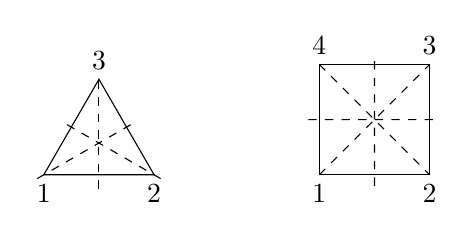
\begin{tikzpicture}[scale=.7]
\draw (0,0)--(2,0)--(1,1.732)--cycle;
\foreach \x/\y/\a/\b in {0/0/1/below,2/0/2/below,1/1.732/3/above}
  \node[\b] at (\x,\y) {$\a$};
\draw[dashed] (1,-.25)--(1,1.73);
\draw[dashed] (-.12,-.07)--(1.65,.95);
\draw[dashed] (2.12,-.07)--(.35,.95);
\begin{scope}[xshift=5cm]
\draw (0,0) rectangle (2,2);
\foreach \x/\y/\a/\b in {0/0/1/below,2/0/2/below,2/2/3/above,0/2/4/above}
  \node[\b] at (\x,\y) {$\a$};
\draw[dashed] (-.2,1)--(2.2,1) (1,-.2)--(1,2.2) (0,0)--(2,2) (0,2)--(2,0);
\end{scope}
\end{tikzpicture}

Gli assi tratteggiati danno le tre riflessioni del triangolo e le quattro del quadrato.
\end{center}

\begin{osservazione}[Sottogruppi diedrali]
Le rotazioni formano il ciclico $\langle r\rangle$. I suoi sottogruppi sono $\langle r^d\rangle$ per $d\mid n$, $d>0$. Ogni riflessione $r^js$ genera un sottogruppo di ordine due, perché $(r^js)^2=r^jr^{-j}=1$. Se un sottogruppo $K$ contiene $r^js$ e $K\cap\langle r\rangle=\langle r^d\rangle$, allora
\[
 K=\langle r^d,r^js\rangle
 =\{r^{td},r^{td+j}s:0\le t<n/d\}.
\]
Infatti il prodotto di una riflessione di $K$ per $r^js$ è una rotazione di $K$, quindi ogni riflessione di $K$ compare nell'elenco. Questo include i sottogruppi $\langle r^d,s\rangle$ delle lezioni.
\end{osservazione}
\Needspace{10\baselineskip}
\begin{esercizio}
Calcolare $Z(S_n)$ per $n\ge3$ e $Z(D_n)$, in particolare per il triangolo e il quadrato.
\end{esercizio}
\begin{svolgimento}
Se $z$ è centrale in $S_n$, allora $(z(i)\ z(j))=(i\ j)$ per ogni trasposizione. Fissato $i$, scegliamo $j,k$ distinti fra loro e da $i$. Ne segue $z(i)\in\{i,j\}\cap\{i,k\}=\{i\}$. Dunque $Z(S_n)=\{1\}$.

In $D_n$ basta commutare con i due generatori. Nessuna riflessione è centrale, perché coniuga $r$ in $r^{-1}\ne r$. La rotazione $r^i$ commuta con $s$ se e solo se $r^i=r^{-i}$, ossia $n\mid 2i$. Per $n$ dispari resta soltanto $1$. Per $n$ pari il centro è $\{1,r^{n/2}\}$, dove il secondo elemento è il mezzo giro. Quindi $Z(D_3)=\{1\}$ e $Z(D_4)=\{1,(1\ 3)(2\ 4)\}$. Benché $D_4\le S_4$, il mezzo giro può essere centrale nel sottogruppo senza esserlo in $S_4$: in generale $Z(G)\cap H\subseteq Z(H)$ per $H\le G$.
\end{svolgimento}

\section{Classi laterali e teorema di Lagrange}
% A–L 23:3–7, 24:1–4; M–Z 23:1–7, 24:1–3.
\begin{definizione}
Per $H\le G$ e $a\in G$, la \textbf{classe laterale destra} $Ha=\{ha:h\in H\}$ si ottiene moltiplicando gli elementi di $H$ a destra per $a$. La \textbf{classe laterale sinistra} è $aH=\{ah:h\in H\}$. In un gruppo abeliano coincidono. In $(\Z,+)$ con $H=m\Z$, $m\ge1$, si ritrovano precisamente le $m$ classi resto $a+m\Z$, $0\le a<m$.
\end{definizione}
\begin{proposizione}
\begin{enumerate}
\item $Ha=Hb$ se e solo se $ab^{-1}\in H$. Per le classi sinistre $aH=bH$ se e solo se $b^{-1}a\in H$.
\item Le classi destre distinte formano una partizione di $G$, come pure le sinistre. Ogni classe ha cardinalità $|H|$.
\end{enumerate}
\end{proposizione}
\begin{proof}
\textbf{1.} Se $Ha=Hb$, allora $a=hb$ per qualche $h\in H$, cioè $ab^{-1}\in H$. Viceversa, se $a=hb$, si ha $Ha=Hhb=Hb$ perché la moltiplicazione per $h$ permuta $H$ con inversa la moltiplicazione per $h^{-1}$. A sinistra lo stesso argomento parte da $a=bh$. Prendendo gli inversi in $H$ si possono anche usare rispettivamente $ba^{-1}$ e $a^{-1}b$. In particolare $Ha=H$ e $aH=H$ precisamente quando $a\in H$. Altrimenti nessuna delle due classi contiene il neutro e quindi nessuna è un sottogruppo.

\textbf{2.} L'uguaglianza $Ha=Hb$ definisce una relazione di equivalenza su $G$. Per il punto 1 la classe di $a$ è $\{b:ba^{-1}\in H\}=Ha$. Il teorema~\ref{teo:partizioni} dà quindi la partizione in classi di equivalenza. A sinistra si procede usando $a^{-1}b\in H$. Le mappe $h\mapsto ha$ e $h\mapsto ah$ sono biezioni da $H$ sulle rispettive classi, con inverse $x\mapsto xa^{-1}$ e $x\mapsto a^{-1}x$.
\end{proof}
L'inversione manda $Ha$ in $a^{-1}H$ e applicata due volte restituisce la classe iniziale. Il numero delle classi destre è dunque quello delle sinistre. Si chiama \textbf{indice} di $H$ in $G$ e si scrive $[G:H]$.
\begin{teorema}[Lagrange]\label{teo:lagrange}
Se $G$ è finito e $H\le G$, allora $|G|=[G:H]|H|$. In particolare $|H|$ divide $|G|$.
\end{teorema}
\begin{proof}
Si scelga un rappresentante per ciascuna classe destra distinta. Le corrispondenti classi sono disgiunte, ricoprono $G$ e contengono ciascuna $|H|$ elementi. Sommando le loro cardinalità si ottiene la formula.
\end{proof}
\begin{esempio}
In $S_3$, per $H=\langle(1\ 2)\rangle$, l'indice è $3$. Oltre a $H$ si hanno
\[
\begin{array}{c|cc}
a&Ha&aH\\\hline
(1\ 3)&\{(1\ 3),(1\ 3\ 2)\}&\{(1\ 3),(1\ 2\ 3)\}\\
(2\ 3)&\{(2\ 3),(1\ 2\ 3)\}&\{(2\ 3),(1\ 3\ 2)\}.
\end{array}
\]
Per $N=\langle(1\ 2\ 3)\rangle$ l'indice è $2$. L'unica classe oltre a $N$, sia a destra sia a sinistra, contiene le tre trasposizioni. In generale, per indice $2$ e $a\notin H$ si ha $Ha=G\setminus H=aH$.
\end{esempio}
\begin{corollario}
\begin{enumerate}
\item In un gruppo finito $\operatorname{ord}(g)\mid |G|$ e $g^{|G|}=1$. Un gruppo di ordine primo è generato da ciascun suo elemento diverso dal neutro.
\item Se $m\ge2$ e $\operatorname{MCD}(a,m)=1$, allora $a^{\varphi(m)}\equiv1\pmod m$ (teorema di Eulero). Per ogni primo positivo $p$ e ogni intero $a$ vale $a^p\equiv a\pmod p$ (piccolo teorema di Fermat).
\end{enumerate}
\end{corollario}
\begin{proof}
\textbf{1.} Applicare Lagrange a $\langle g\rangle$, che ha cardinalità $d=\operatorname{ord}(g)$. Scrivendo $|G|=dq$ segue $g^{|G|}=(g^d)^q=1$. Se $|G|=p$ e $g\ne1$, l'unico divisore possibile per $d>1$ è $p$, quindi $\langle g\rangle=G$.

\textbf{2.} Applicare il punto 1 al gruppo moltiplicativo delle unità modulo $m$, che contiene $[a]_m$ ed ha $\varphi(m)$ elementi. Per $m=p$ primo e $p\nmid a$, moltiplicare $a^{p-1}\equiv1\pmod p$ per $a$. Se $p\mid a$, entrambi i membri di $a^p\equiv a\pmod p$ sono congrui a zero.
\end{proof}
\begin{esempio}[I conversi di Lagrange]
In $S_5$ non esiste alcun sottogruppo di ordine $7$ perché $7\nmid120$. La divisibilità, quando vale, può non bastare. In $S_3$ nessun elemento ha ordine $6$. In $S_4$ gli ordini possibili sono $1,2,3,4$, come si legge dalle partizioni di $4$ in lunghezze di cicli. In particolare manca un elemento di ordine $12$, mentre esiste un sottogruppo di ordine $12$, ossia $A_4$. Anzi tutti i divisori di $24$ sono ordini di sottogruppi: per $1,2,3,4$ bastano i ciclici, per $6$ le permutazioni che fissano $4$, per $8$ il gruppo del quadrato, per $12,24$ i gruppi $A_4,S_4$. Nel caso di un gruppo ciclico finito il converso vale anche per gli elementi, come segue dalla classificazione dei suoi sottogruppi.
\end{esempio}
